\subsection{Fill-In}

\begin{flushleft}
    \textcolor{Green3}{\faIcon{question-circle} \textbf{What is the fill-in?}}
\end{flushleft}
When performing LU decomposition on a sparse matrix $A$, the resulting matrices $L$ (lower triangular) and $U$ (upper triangular) may have non-zero elements in positions that were originally zero in $A$. This phenomenon is called fill-in.

\highspace
\begin{flushleft}
    \textcolor{Red2}{\faIcon{exclamation-triangle} \textbf{Impact}}
\end{flushleft}
Fill-in \textbf{increases the storage requirements and computational complexity} of the decomposition. 

\highspace
\begin{flushleft}
    \textcolor{Green3}{\faIcon{book} \textbf{Fill-In Reduction Strategies}}
\end{flushleft}
To reduce fill-in, reordering techniques are employed. This involves renumbering the rows of $A$ differently to minimize the number of non-zero elements in $L$ and $U$.
\begin{itemize}
    \item \important{Permutation Matrix $P$}. Reordering can be achieved by pre-multiplying $A$ by a permutation matrix $P$, which swaps rows to achieve a more favorable structure.
\end{itemize}
\begin{figure}[!htp]
    \centering
    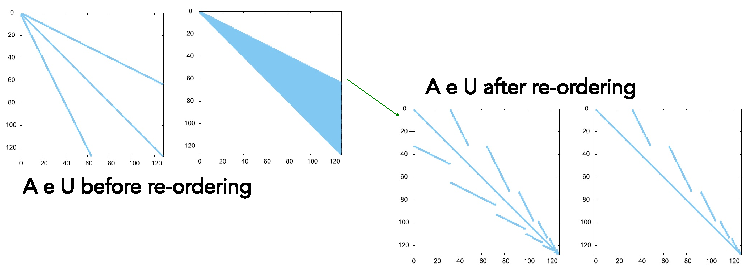
\includegraphics[width=\textwidth]{img/fill-in-1.pdf}
\end{figure}